

\definecolor{dkgreen}{rgb}{0,0.6,0}
\definecolor{gray}{rgb}{0.5,0.5,0.5}
\definecolor{mauve}{rgb}{0.58,0,0.82}

\lstdefinestyle{customc}{
  belowcaptionskip=1\baselineskip,
  breaklines=true,
  frame=L,
  xleftmargin=\parindent,
  language=C,
  showstringspaces=false,
  basicstyle=\footnotesize\ttfamily,
  keywordstyle=\bfseries\color{green!40!black},
  commentstyle=\itshape\color{purple!40!black},
  identifierstyle=\color{blue},
  stringstyle=\color{orange},
}

\lstdefinestyle{customasm}{
  belowcaptionskip=1\baselineskip,
  frame=L,
  xleftmargin=\parindent,
  language=[x86masm]Assembler,
  basicstyle=\footnotesize\ttfamily,
  commentstyle=\itshape\color{purple!40!black},
}

\lstset{escapechar=@,style=customc}

\subsection{Modulacja szerokości impulsu (PWM)}
Implementacja PWM umożliwia precyzyjne sterowanie elementami wykonawczymi wymagającymi sygnału analogowego, takimi jak silniki czy regulacja jasności diody LED. Funkcjonalność obejmuje konfigurację częstotliwości sygnału PWM, ustawianie wypełnienia impulsu (duty cycle) oraz dynamiczną zmianę parametrów w zależności od warunków środowiskowych. PWM jest wykorzystywane do regulacji intensywności świecenia diod LED w diodzie RGB LED3 [schemat]. %dodaj schemat
W projekcie został wykorzystany PWM1.

\subsubsection{Inicjalizacja PWM1}
\begin{enumerate}
    \item Konfigurację rozpoczynamy od włączenia zasilania. W tym celu ustawiamy 6 bit w rejestrze PCONP (tabela 46.) %odwolanie do dokumentacji
    \item Piny na których chcemy sterować impulsami to P2.0, P2.1, P2.2. Chcemy je ustawić jako PWM1.1, PWM1.2, PWM1.3, dlatego w rejestrze PINSEL4 ustawiamy bity 1:0, 3:2, 5:4 na 01 - funkcja PWM1.X
    % \item Następnie wybieramy tryb pracy na single edge, czyli
    \item Opis rejestrów PWM1:\\
    \begin{enumerate}
        \item \textbf{IR} - rejestr ten służy do zarządzania przerwaniami. Przerwania 
        \begin{enumerate}
            \item \textbf{PWMMR0 Interrupt} - bit 0, flaga przerwania na kanale 0
            \item \textbf{PWMMR1 Interrupt} - bit 1, flaga przerwania na kanale 1
            \item \textbf{PWMMR2 Interrupt} - bit 2, flaga przerwania na kanale 2
            \item \textbf{PWMMR3 Interrupt} - bit 3, flaga przerwania na kanale 3
            \item \textbf{PWMCAP0 Interrupt} - bit 4, flaga przerwania dla zerowego wejscia przechwytującego (capture input); capture oznacza przechwycenie aktualnej wartości licznika (timer'a), np. w momencie zbocza sygnału (narastającego lub opadającego) na pinie wejściowym. Umożliwia to np. pomiar czasu trwania impulsów, okresów czy częstotliwości.
            \item \textbf{PWMCAP1 Interrupt} - bit 5, flaga przerwania dla pierwszego wejscia przechwytującego 
            \item Bity 7:6 - zarezerwowane
            \item \textbf{PWMMR4 Interrupt} - bit 8, flaga przerwania na kanale 4
            \item \textbf{PWMMR5 Interrupt} - bit 9, flaga przerwania na kanale 5
            \item \textbf{PWMMR6 Interrupt} - bit 10, flaga przerwania na kanale 6
            \item Bity 31:11 - zarezerwowane

        \end{enumerate}
        \item \textbf{PWM1TCR}
        \begin{enumerate}
            \item \textbf{Counter Enable} - bit 0, włączanie i wyłączanie licznika timera oraz preskalera
            \item \textbf{Counter Reset} - bit 1, resetowanie licznika timera, synchoronizacja z kolejnym zboczem narastającym PCLK, tak długo, aż wartość tego bitu będzie równa 1
            \item Bit 2 - zarezerwowany
            \item \textbf{PWM Enable} - gdy wartość bitu jest róna 1 - \textbf{tryb PWM}, licznik resetuje się do 1, aktywuje shadow registery.\\
                            Gdy wartość bitu jest równa 0 - \textbf{tryb timer}, licznik resetuje się do 0, bez PWM - działą jak zwykły timer.
            \item Bit 4:31 - zarezerwowane
        \end{enumerate}
        \item \textbf{PWM1CTCR} - rejestr służy do wyboru trybu licznika - timer lub jako licznik zliczający impulsy z zewnętrznego źródła. 
        \begin{enumerate}
            \item \textbf{Counter/Timer Mode} - bity 0:1, wartości i odpowiadające im działanie zostały opisane w poniższej tabeli.
            \begin{table}[H]
                \centering
                \begin{tabular}{|c|p{13cm}|}
                    \hline
                    \rowcolor{gray!30}
                    Wartość & Opis\\
                    \hline
                    00  & Timer mode: Timer Counter (TC) wykorzystuje Prescale Counter (PC) oraz Prescale Register (PR), aby móc działać wolniej. TC inkrementuje się gdy PC = PR\\
                    \hline
                    01 & Counter Mode: TC zlicza impulsy przychodzące (inkrementacja przy każdym zboczu narastającym) z zewnętrznego pinu wybranego na bitach 3:2  \\
                    \hline
                    10 & Counter Mode: TC zlicza impulsy przychodzące (inkrementacja przy każdym zboczu opadającym) z zewnętrznego pinu wybranego na bitach 3:2  \\
                    \hline
                    11 & Counter Mode: TC zlicza impulsy przychodzące (inkrementacja przy na obu zboczach impulsu) z zewnętrznego pinu wybranego na bitach 3:2  \\
                    \hline
                \end{tabular}
                \caption{Rodzaje pracy w trybie Timer/Counter}
            \end{table}
            \item \textbf{Count Input Select} - bity 3:2 - ta częśćrejestru odpowiada za wybó pinu PCAP z którego będą zliczane impulsy.\\
            \begin{table}[H]
                \centering
                \begin{tabular}{|c|p{13cm}|}
                    \hline
                    \rowcolor{gray!30}
                    Wartość & Opis\\
                    \hline
                    00  & Timer mode: Timer Counter (TC) wykorzystuje Prescale Counter (PC) oraz Prescale Register (PR), aby móc działać wolniej. TC inkrementuje się gdy PC = PR\\
                    \hline
                    01 & Counter Mode: TC zlicza impulsy przychodzące (inkrementacja przy każdym zboczu narastającym) z zewnętrznego pinu wybranego na bitach 3:2  \\
                    \hline
                    10 & Counter Mode: TC zlicza impulsy przychodzące (inkrementacja przy każdym zboczu opadającym) z zewnętrznego pinu wybranego na bitach 3:2  \\
                    \hline
                    11 & Counter Mode: TC zlicza impulsy przychodzące (inkrementacja przy na obu zboczach impulsu) z zewnętrznego pinu wybranego na bitach 3:2  \\
                    \hline
                \end{tabular}
                \caption{Rodzaje pracy w trybie Timer/Counter}
            \end{table}
            
            \item \textbf{PWM1MCR} - steruje reakcjami układu PWM, gdy zawartość rejestru licznika czasowego PWM Timer Counter (TC) jest równa jednej z wartości w rejestrach dopasowania PWM Match Registers (MR0–MR6). Ustawienie jedynki na poniższych bitach powoduje włączenie danej funkcji.
            \begin{enumerate}
                \item \textbf{PWMMR0I} - bit 0, gdy rejestr licznika PWM (PWM Timer Counter) osiągnie wartość ustawioną w Match Register 0 – PWMMR0, może wystąpić przerwanie - jeśli wartość ustawiona na tym bicie to 1
                \item \textbf{PWMMR0R} - bit 1, gdy zawartość licznika PWMTC jest równa wartości PWMMR0 nastąpi reset PWMTC; Pozwala to tworzyć cykliczny sygnał PWM – licznik odlicza od 0 do wartości w PWMMR0, potem reset.
                \item \textbf{PWMMR0S} - bit 3, zatrzymuje licznik, gdy wartość w rejestrze PWMTC jest równa wartości zapisanej w PWMMR0
                \item funkcjonalności kolejnych bitów tego rejestru są cyklicznie powtarzane dla PWMMR1f, PWMMR2f, PWMMR3f, PWMMR4f, PWMMR5f, PWMMR6f (gdzie 'f' oznacza numer rejestru PWMMR)\\
                                        Bity 21:31 są zarezerwowane.
            \end{enumerate}

            \item \textbf{PWM1CCR} - rejestr pozwala skonfigurować zdarzenia przechwytywania (capture events) na wejściach CAPn.x, czyli kiedy wartość licznika zostanie zapisana do rejestru przechwytywania (CRn), gdzie n jest numerem Timera - 0 lub 1. Warto zaznaczyć, że jeśli CAP input jest skonfigurowane jako źródło zliczania (Counter Mode w CTCR), to jego bity w PWM1CCR muszą mieć wartość 000.
                Poniższe funkcje są dostępne przy ustawieniu flagi na 1 we wskazanym bicie.
                \begin{enumerate}
                    \item \textbf{Capture on CAPn.0 rising edge} - bit 0, jeśli zostanie wykryte zbocze narastające, to do rejestru przechwytywania CR0 zostanie wpisana zawartość TC
                    \item \textbf{Capture on CAPn.0 falling edge} - bit 1, jeśli zostanie wykryte zbocze opadające, to do rejestru przechwytywania CR0 zostanie wpisana zawartość TC
                    \item \textbf{Interrupt on CAPn.0 event} - bit 3, jeśli zostanie wykryte zdarzenie przechwycenia, to zawartośćTC zostanie wpisana do CR0 oraz zostanie wygenerowane przewanie
                    \item Takie same funkcje mają bity 5:3, ale dla CAPn.1 i zapis do CR1.
                    \item Bity 31:6 są zarezerwowane.
                \end{enumerate}
            \item \textbf{PWM1PCR} - rejestr służy do włączania PWM oraz wybierania trybu działąnia kanału.
                \begin{enumerate}
                    \item \textbf{PWMSELx} - wybór trybu pracy dla kanału PWMx, gdzie x to numery 2-6.\\
                        Poniższa tabela opisuje generowany impuls w zależności od ustawionego bitu. \\
                        Bity 0:1 sąnieużywane, zawsze mają wartość 0.\\
                        Bity 7:8 - są zarezerwowane.\\
                        Zatem bity ustawiające tryby pracy to 6:2.
                        \begin{table}[H]
                            \centering
                            \begin{tabular}{|c|c|p{10cm}|}
                                \hline
                                \rowcolor{gray!30}
                                Wartość & Tryb & Opis\\
                                \hline
                                    0 & Single-edge & Generowany jest impuls z jedną \hyperref[fig:single-edge-left-pwm]{krawędzią opadającą}, ponieważ z \href{https://www.zsk.p.lodz.pl/~morawski/SCR&ES/NotyKatalogowe/UM10360.pdf#page=119&zoom=100,210,814}{dokumentacji (strona 520)}., wynika iż każdy cykl PWM zaczyna się od stanu wysokiego.\\
                                \hline
                                    1 & Double-edge & Generowany jest impuls z \hyperref[fig:double-edge-center-pwm]{dwiema krawędziami} (umożliwia symetryczne impulsy)\\
                                \hline
                            \end{tabular}
                            \caption{Rodzaje pracy w trybie Timer/Counter}
                        \end{table}

                        \begin{figure}[H]
                            \centering
                            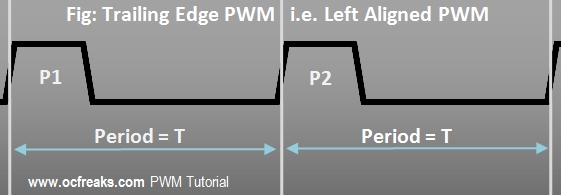
\includegraphics[width=0.8\textwidth]{../PWM/single_edge_left.jpg}
                            \caption{Przedstawienie trybu single-edge PWM, lewy impuls}
                            \label{fig:single-edge-left-pwm}
                        \end{figure}

                        \begin{figure}[H]
                            \centering
                            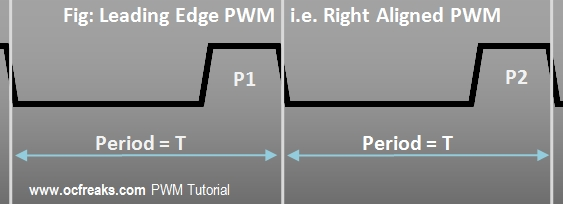
\includegraphics[width=0.8\textwidth]{../PWM/single_edge_right.jpg}
                            \caption{Przedstawienie trybu single-edge PWM, prawy impuls}
                            \label{fig:single-edge-right-pwm}
                        \end{figure}

                        \begin{figure}[H]
                            \centering
                            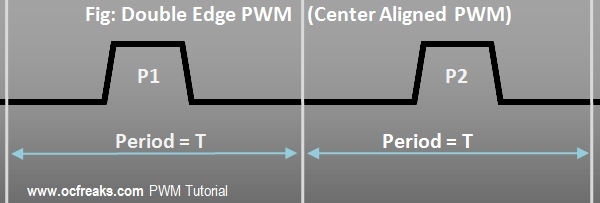
\includegraphics[width=0.8\textwidth]{../PWM/double-edge-center-pwm.jpg}
                            \caption{Przedstawienie trybu double-edge PWM}
                            \label{fig:double-edge-center-pwm}
                        \end{figure}
                    
                        \item \textbf{PWMENAx} - służy do włączania lub wyłączania wyjścia PWM, gdzie x to numer kanału PWM (1-6). Ustawianie tych funkcji odbywa się na bitach 14:9. Wartość 1 włącza wyjście, a wartość 0 wyłącza. Bity 15:31 są nieużywane i mają wartość 0.
                        \item \textbf{PWM1LER} - używany jest do aktualizacji rejestró PWM Match, ponieważ w trybie PWM Mode, wartości wpisywane do rejestrów dopasowania nie są od razu używane, ale trafiają do rejestrów tymczasowych (shadow registers). Zmiany należy zatwierdzić poprzez ustawienie odpowiednich bitó w PWM1LER. Zmiany są widoczne dopiero po rozpocząciu nowego cyklu PWM.
                        %MR0 - sufit - koniec cyklu
                        %MRx (x = 1–6) = moment zbocza opadającego
                        %W trybie single edge: zbocze narastające zawsze w 0
                        %W double edge: zbocza mogą być ustawione niezależnie w MRx i MRy (np. MR1 i MR2)
                \end{enumerate}
            
                

        \end{enumerate}

        
    \end{enumerate}

    \item Omówienie zagadnienia PWM na podstawie sterowania diodą LED3. \\
        LED3, to dioda RGB, skłądająca się z oddzielnych diod czerwonej, zielonej i niebieskiej (wspólny plus). Wykorzystanie PWM do pośredniego (sterujemy masą poprzez tranzystory \hyperref[fig:led3]{(schemat)}) sterowania jasnością diod RGB umożliwia dostosowanie jasności poszczególnych kolorów w zależności od potrzeb.
        \begin{figure}[H]
            \centering
            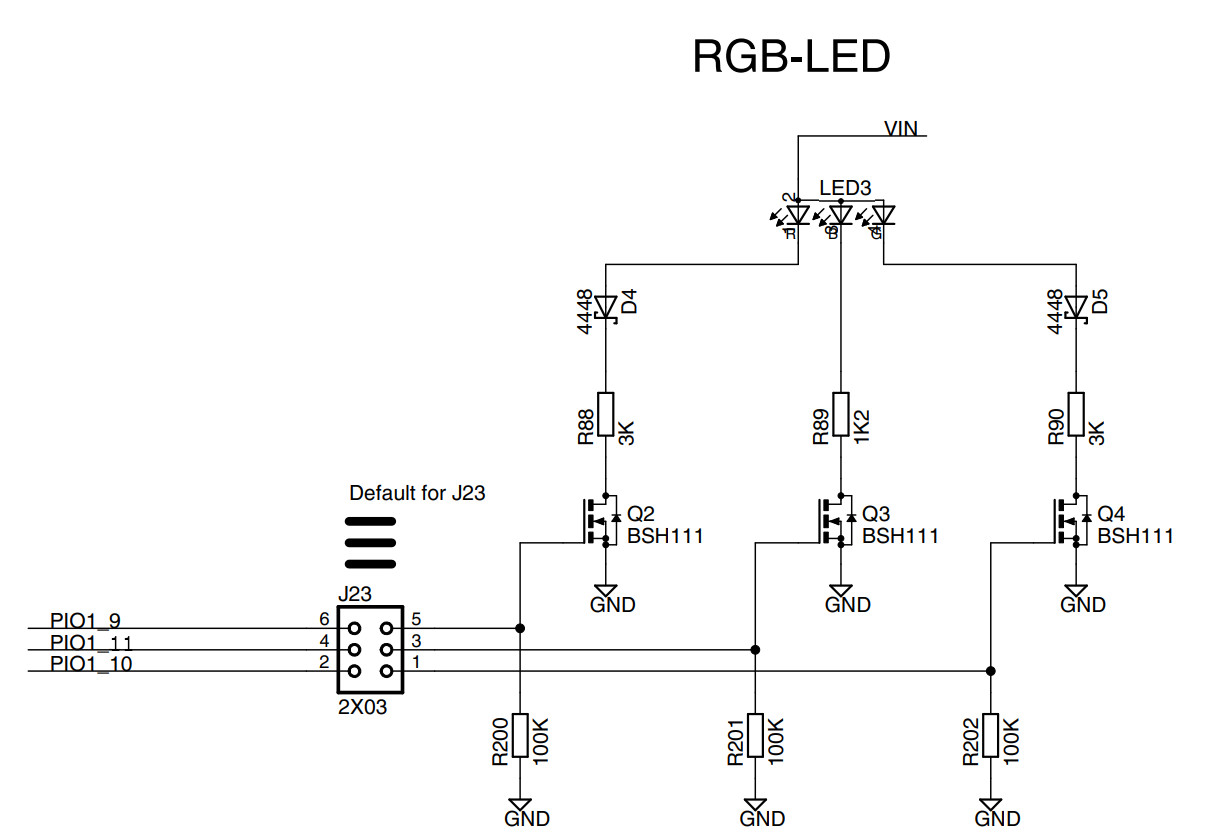
\includegraphics[width=0.8\textwidth]{../PWM/led3.jpg}
            \caption{Schemat diody RGB}
            \label{fig:led3}
        \end{figure}
        
        Jasność diody jest skorelowana z szerokością impulsu. Ze względu na zapis szestnastkowy kolorów RGB (każdy kolor ma zakres 0-255), zdecydowaliśmy się na okres 255.
        \begin{lstlisting}
LPC_PWM1->PCR = (1 << 9) | (1 << 10) | (1 << 11);  // ustawiamy tryb PWM na single-edge

LPC_PWM1->PR = 0;         // TC jest inkrementowany przy PR+1, wiec dzielnik zegara sie nie zmienia. 
                          // Czestotliwosc wynosi 25 MHz / 1 = 25 MHz
LPC_PWM1->MR0 = 255;      // Okres PWM = 255 cykli 
LPC_PWM1->MCR = (1 << 1); // Reset na MR0 (PWM cycle)

LPC_PWM1->MR1 = 255;      // Ustawiamy jasnosc na 100%, szerokosc impulsow = 255 / 255 = 100%
LPC_PWM1->MR2 = 255;      
LPC_PWM1->MR3 = 255; 

LPC_PWM1->LER = (1 << 1) | (1 << 2) | (1 << 3) | (1 << 0); // Aktualizacja rejestrow MRx

LPC_PWM1->TCR = (1 << 0) | (1 << 3);  // Wlaczamy PWM
        \end{lstlisting}

        Kolor LED3 ustawiamy przy pomocy funkcji $PWM_SetColor(uint8_t red, uint8_t green, uint8_t blue)$, która zmienia zawartość rejestrów MR1, MR2 i MR3.
        
        \begin{lstlisting}
void PWM_SetColor(uint8_t red, uint8_t green, uint8_t blue) {
    if( red < 0 || red > 255 ) return; // ograniczenie zakresu
    if( green < 0 || green > 255 ) return;
    if( blue < 0 || red > 255 ) return;

    LPC_PWM1->MR1 = red; // ustawiamy szerokosc impulsu dla diody czerwonej
    LPC_PWM1->MR2 = blue; // ustawiamy szerokosc impulsu dla diody niebieskiej
    LPC_PWM1->MR3 = green; // ustawiamy szerokosc impulsu dla diody zielonej

    LPC_PWM1->LER = (1 << 1) | (1 << 2) | (1 << 3);  // zaktualizuj MR1-MR3
}
        \end{lstlisting}
\end{enumerate}
